\section{Underlying Principles}
\label{appendix:principles}
The INTO-CPS tool chain facilitates the design and validation of CPSs through its implementation of results from a number of underlying principles.
%
These principles are co-simulation, design space exploration, model-based test automation and code generation.
%
This appendix provides an introduction to these concepts.
%
%
%
\subsection{Co-simulation}
Co-simulation refers to the simultaneous simulation of individual models which together make up a larger system of interest, for the purpose of obtaining a simulation of the larger system.
%
A co-simulation is performed by a co-simulation orchestration engine.
%
This engine is responsible for initializing the individual simulations as needed;  for selecting correct time step sizes such that each constituent model can be simulated successfully for that duration, thus preventing time drift between the constituent simulations;  for asking each individual simulation to perform a simulation step;  and for synchronizing information between models as needed after each step.
%
The result of one such round of simulations is a single simulation step for the complete multi-model of the system of interest.

As an example, consider a very abstract model of a nuclear power plant.
%
This consists of a nuclear reactor core, a controller for the reactor, a water and steam distribution system, a steam-driven turbine and a standard electrical generator.
%
All these individual components can be modelled separately and simulated, but when composed into a model of a nuclear power plant, the outputs of some become the inputs of others.
%
In a co-simulation, outputs are matched to inputs and each component is simulated one step at a time in such a way that when each model has performed its simulation step, the overall result is a simulation step of the complete power plant model.
%
Once the correct information is exchanged between the constituent models, the process repeats.
%
%
%
\subsection{Design Space Exploration}
During the process of developing a CPS, either starting from a completely blank canvas or constructing a new system from models of existing components, the architects will encounter many design decisions that shape the final product.
%
The activity of investigating and gathering data about the merits of the different choices available is termed Design Space Exploration.
%
Some of the choices the designer will face could be described as being the selection of parameters for specific components of the design, such as the exact position of a sensor, the diameter of wheels or the parameters affecting a control algorithm.
%
Such parameters are variable to some degree and the selection of their value will affect the values of objectives by which a design will be measured.
%
In these cases it is desirable to explore the different values each parameter may take and also different combinations of these parameter values if there are more than one parameter, to find a set of designs that best meets its objectives.
%
However, since the size of the design space is the product of the number of parameters and the number of values each may adopt, it is often impractical to consider performing simulations of all parameter combinations or to manually assess each design.

The purpose of an automated DSE tool is to help manage the exploration of the design space, and it separates this problem into three distinct parts:  the search algorithm, obtaining objective values and ranking the designs according to those objectives.
%
The simplest of all search algorithms is the exhaustive search, and this algorithm will methodically move through each design, performing a simulation using each and every one.
%
This is termed an open loop method, as the simulation results are not considered by the algorithm at all.
%
Other algorithms, such as a genetic search, where an initial set of randomly generated individuals are bred to produce increasingly good results, are closed loop methods.
%
This means that the choice of next design to be simulated is driven by the results of previous simulations.

Once a simulation has been performed, there are two steps required to close the loop.
%
The first is to analyze the raw results output by the simulation to determine the value for each of the objectives by which the simulations are to be judged.
%
Such objective values could simply be the maximum power consumed by a component or the total distance traveled by an object, but they could also be more complex measures, such as the proportion of time a device was operating in the correct mode given some conditions.
%
As well as numerical objectives, there can also be constraints on the system that are either passed or failed.
%
Such constraints could be numeric, such as the maximum power that a substation must never exceed, or they could be based on temporal logic to check that undesirable events do not occur, such as all the lights at a road junction not being green at the same time.
%

The final step in a closed loop is to rank the designs according to how well each performs.
%
The ranking may be trivial, such as in a search for a design that minimizes the total amount of energy used, or it may be more complex if there are multiple objectives to optimize and trade off.
%Unless there is a trivial goal for the system, such as simply minimising energy used, then there is a need for the final part of closed loop, which is to rank designs according to their objective values and their ability to meet the constraints set out for them.
%
Such ranking functions can take the form of an equation that returns a score for each design, where the designs with the highest/lowest scores are considered the best.
%
Alternatively, if the relationship between the desired objectives is not well understood, then a Pareto approach can be taken to ranking, where designs are allocated to ranks of designs that are indistinguishable from each other, in that each represents an optimum, but there exist different tradeoffs between the objective values.  
%
%
%
\subsection{Model-Based Test Automation}
The core fragment of test automation activities is a model of the desired system behaviour, which can be expressed in SysML.
%
This test model induces a transition relation, which describes a collection of execution paths through the system, where a path is considered a
sequence of timed data vectors (containing internal data, inputs and outputs).
%
The purpose of a test automation tool is to extract a subset of these paths from the test model and turn these paths into test
cases, respectively test procedures.
%
The test procedures then compare the behaviour of the actual system-under-test to the path, and produce warnings once discrepancies are observed.
%
%
%
%\subsection{Model Checking}
%Naturally, model checking applied to a co-simulation environment is not dissimilar to model checking of distributed systems, which are formed from independent components. 
%%
%The purpose is to verify properties of the entire system, consisting of numerous components that run in parallel.
%%
%There is one important dissimilarity, however.  In INTO-CPS, the system structure consists of heterogeneous models, and these different components may be specified using different formalisms, or the entire system may even employ simulations, auto-generated code and real hardware controllers.
%%
%This observation leads to the need for a uniform representation of models -- no matter how they are implemented -- that can be used for model checking purposes, and naturally, for a precise notion of abstraction.
%
%To apply model checking to an INTO-CPS multi-model, there is one more challenge when integrating components of different kinds.
%%
%Some of the components may, for example, depend on the calculation of differential equations, for which model checking is intractable except for the smallest examples.
%%
%The drive to analyze and verify real-world systems thus forces us to represent complex components by their abstract counterparts, which are again expressed as timed state charts.
%%
%That is, all models need to be represented as discrete event models.
%
%The key idea in abstraction is to represent a concrete model $\mathcal{M}$ by a more abstract counterpart $\alpha(\mathcal{M})$ by application of an abstraction function $\alpha$.
%%
%In essence, $\alpha$ must be designed so that $\alpha(\mathcal{M})$ describes all behaviours originally presented in $\mathcal{M}$, and possibly additional ones.
%%
%Thus, abstraction preserves safety properties: If a safety property holds for the abstract model
%$\alpha(\mathcal{M})$, then the property also holds for the concrete model $\mathcal{M}$.
%%
%However, since $\alpha$ may introduce additional behaviours, checking $\alpha(\mathcal{M})$ may lead to false positive warnings: a property
%violation may be reported for $\alpha(\mathcal{M})$, but the violated behaviour is not part of the concrete model $\mathcal{M}$. Details on how $\alpha$ can be implemented are described in~\cite{INTOCPSD51c}.
%
%Apart from the need for abstraction, the topology of the model connection is more involved for co-simulation as implemented in INTO-CPS.
%%
%The overall system design does not consist of a single system-under-test, but rather a collection of systems whose inputs and outputs are connected using a graph-like structure.
%
%With respect to the turn indication example from Section~\ref{appendix:rtt-model-checking} (Figure~\ref{figure:vsi-simple}), the same behaviour may be implemented by two independent controllers, one for each side.
%%
%Then, the overall system topology is connected as given in Fig.~\ref{figure:vsi-more-complex}.
%%
%By using this kind of modelling, where different system models are all included as timed state charts, it is possible to specify LTL formulae as before.
%%
%This form of modelling connections between system components, however, is an integral part of the INTO-CPS project.
%%
%Model checking in the context of INTO-CPS thus smoothly integrates with the overall INTO-CPS approach.
%%
%%
%%
%\begin{figure}
%\centerline{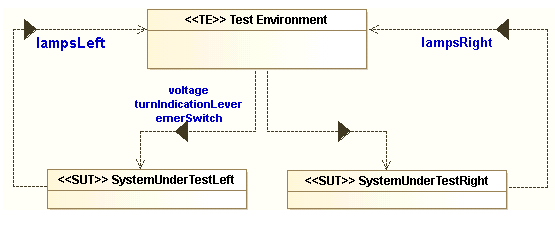
\includegraphics[width=\textwidth]{figures/VSI-modelio-more-complex.png}}
%\caption{Extension of the system topology sketched in
%  Fig.~\ref{figure:vsi-simple}.}
%\label{figure:vsi-more-complex}
%\end{figure}
%
%
%
\subsection{Code Generation}
Code generation refers to the translation of a modelling language to a common programming language.
%
Code generation is commonly employed in control engineering, where a controller is modelled and validated using a tool such as 20-sim, and finally translated into source code to be compiled for some embedded execution platform, which is its final destination.

The relationship that must be maintained between the source model and translated program must be one of refinement, in the sense that the translated program must not do anything that is not captured by the original model.
%
This must be considered when translating models written in high-level specification languages, such as VDM.
%
The purpose of such languages is to allow the specification of several equivalent implementations.
%
When a model written in such a language is translated to code, one such implementation is essentially chosen.
%
In the process, any non-determinism in the specification, the specification technique that allows a choice of implementations, must be resolved.
%
Usually this choice is made very simple by restricting the modelling language to an executable subset, such that no such non-determinism is allowed in the model.
%
This restricts the choice of implementations to very few, often one, which is the one into which the model is translated via code generation.
